\begin{table}[t]
    \centering
    \caption{Models performance on Skype data}
    \label{class-skype}
%    \resizebox{\columnwidth}{!}{
    \begin{tabular}{|l|l|l|l|l|}
        \hline
        \textbf{Model} & \textbf{Precision (\%)} & \textbf{Accuracy (\%)} & \textbf{Recall (\%)} & \textbf{MSE} \\ \hline
        SVR      & 89.33                      & 89.33                   & 89.33                     & 0.36                 \\ \hline
        MLP      & 90.77                      & 90.77                   & 89.62                     & 0.36                  \\ \hline
        KNN      & 82.91                      & 81.67                   & 81.67                     & 0.63                  \\ \hline
        RF       & 89.72                      & 89.34                   & 89.34                     & 0.41                  \\ \hline
        ADT       & 92.21                      & 92.00                   & 92.00                     &0.29                   \\ \hline 
    \end{tabular}
%    }
\end{table}

\begin{table}[t]
    \centering
    \caption{Models performance on FaceTime data}
    \label{class-facetime}
%    \resizebox{\columnwidth}{!}{
    \begin{tabular}{|l|l|l|l|l|}
        \hline
        \textbf{Model} & \textbf{Precision (\%)} & \textbf{Accuracy (\%)} & \textbf{Recall (\%)} & \textbf{MSE} \\ \hline
        SVR      & 88.13                   & 86.00                  & 86.00                &  0.32                 \\ \hline
        MLP      & 90.00                   & 89.77                  & 89.30                &  0.28                 \\ \hline
        KNN      & 74.98                   & 72.00                  & 72.30                &  0.48                 \\ \hline 
        RF       & 90.37                   & 90.00                  & 90.00                &  0.28                 \\ \hline 
        ADT       & 90.28                   & 90.00                  & 90.00                & 0.26                  \\ \hline 
    \end{tabular}
%    }
\end{table}

\begin{table}[t]
    \centering
    \caption{Models performance on Hangouts data}
    \label{class-hangouts}
%    \resizebox{\columnwidth}{!}{
    \begin{tabular}{|l|l|l|l|l|}
        \hline
        \textbf{Model} & \textbf{Precision (\%)} & \textbf{Accuracy (\%)} & \textbf{Recall (\%)} & \textbf{MSE} \\ \hline
        SVR            & 91.36                        & 90.67                       & 90.67                     & 0.44                  \\ \hline
        MLP            & 89.34                        & 88.48                       & 88.48                     & 0.45                  \\ \hline
        KNN       & 87.02                        & 86.67                       & 86.67                     & 0.49                  \\ \hline 
        RF       & 91.22                        & 90.67                       & 90.67                     &  0.43                 \\ \hline 
        ADT       & 93.75                        & 93.33                       & 93.33                     & 0.38                  \\ \hline 
    \end{tabular}
%    }
\end{table}

\begin{table}[t]
\centering
\caption{Model performance across devices for Skype}
\label{label:skype-devices}
%    \resizebox{\columnwidth}{!}{
    \begin{tabular}{|c|c|c|c|c|}
\hline
\multicolumn{2}{|c|}{Devices}                & \multicolumn{3}{c|}{Model Performance}             \\ \hline
    \multicolumn{1}{|c|}{Training} & Testing     & \multicolumn{1}{c|}{Precision (\%)} & {Accuracy (\%)} & {Recall (\%)} \\ \hline
\multirow{3}{*}{SG-S6 Phone}   & SG-S6 Phone & 89.90  & 88.57 & 88.57       \\ \cline{2-5} 
                               & SG-S2 Tab   & 88.41  & 88.00 & 88.00       \\ \cline{2-5} 
                               & Pixel Tab   & 88.52  & 87.62 & 87.62       \\ \hline
\multirow{3}{*}{SG-S2 Tab}     & SG-S6 Phone & 83.73  & 84.43 & 83.00       \\ \cline{2-5} 
                               & SG-S2 Tab   & 93.04  & 91.43 & 91.43       \\ \cline{2-5} 
                               & Pixel Tab   & 82.69  & 82.86 & 82.86       \\ \hline
\multirow{3}{*}{Pixel Tab}     & SG-S6 Phone & 84.43  & 84.00 & 84.00       \\ \cline{2-5} 
                               & SG-S2 Tab   & 84.40  & 86.49 & 86.49       \\ \cline{2-5} 
                               & Pixel Tab   & 88.20  & 94.40 & 94.00       \\ \hline
\end{tabular}
%}
\end{table}

\begin{table}[t]
\centering
\caption{Model performance across devices for FaceTime}
\label{label:facetime-devices}
%    \resizebox{\columnwidth}{!}{
\begin{tabular}{|c|c|c|c|c|}
\hline
\multicolumn{2}{|c|}{Devices}                & \multicolumn{3}{c|}{Model Performance}             \\ \hline
    \multicolumn{1}{|c|}{Training} & Testing     & \multicolumn{1}{c|}{Precision (\%)} & {Accuracy (\%)} & {Recall (\%)} \\ \hline
\multirow{3}{*}{iPad Pro}   & iPad Pro & 93.60  & 92.00 &   92.00     \\ \cline{2-5} 
                               & iPhone 8 Plus & 90.18  & 89.93 & 89.93       \\ \hline
\multirow{3}{*}{iPhone 8 Plus}     & iPad  Pro  & 88.34  & 88.34  & 88.34       \\ \cline{2-5}  
                               & iPhone 8 Plus  & 92.50  & 92.00 & 92.00       \\ \hline
\end{tabular}
%}
\end{table}

\begin{table}[t]
\centering
\caption{Model performance across devices for Hangouts}
\label{label:hangouts-devices}
%    \resizebox{\columnwidth}{!}{
\begin{tabular}{|c|c|c|c|c|}
\hline
\multicolumn{2}{|c|}{Devices}                & \multicolumn{3}{c|}{Model Performance}             \\ \hline
    \multicolumn{1}{|c|}{Training} & Testing     & \multicolumn{1}{c|}{Precision (\%)} & {Accuracy (\%)} & {Recall (\%)} \\ \hline
\multirow{3}{*}{SG-S6 Phone}   & SG-S6 Phone & 90.03  & 90.00 & 90.00       \\ \cline{2-5} 
                               & SG-S2 Tab   & 84.26  & 84.77 & 84.77       \\ \cline{2-5} 
                               & Pixel Tab   & 82.86  & 82.00 & 82.00       \\ \hline
\multirow{3}{*}{SG-S2 Tab}     & SG-S6 Phone & 89.61  & 89.21 & 89.21       \\ \cline{2-5} 
                               & SG-S2 Tab   & 91.76  & 90.00 & 90.00       \\ \cline{2-5} 
                               & Pixel Tab   & 85.41  & 84.77 & 84.77       \\ \hline
\multirow{3}{*}{Pixel Tab}     & SG-S6 Phone & 86.79  & 86.00 & 86.00       \\ \cline{2-5} 
                               & SG-S2 Tab   & 85.05  & 85.00 & 85.00       \\ \cline{2-5} 
                               & Pixel Tab   & 86.17  & 86.67 & 86.67       \\ \hline
\end{tabular}
%}
\end{table}

\subsection{Modeling Our Metrics to MOS} \label{label:model}

We now present our MOS prediction model that corroborates that our metrics accurately capture QoE artefacts and users' MOS. We build a model to map our objective metrics to subjective evaluations (MOS from user-study). Typically network administrators need to estimate a subjective evaluation such as MOS. However, QoE assignment in 5 classes can be cumbersome and may give little information on network quality. Hence, we map MOS scores to 3 classes (i.e., bad, average, good) that can be used by LTE or WiFi deployments to enhance resource allocation. We first explain our modeling methodology from freeze and blur metrics to MOS, and then describe how to translate MOS into 3-class QoE.

Typically, objective QoE metrics are mapped to MOS scores using non-linear regression \cite{cui2008image}. 
Our regression model employs the average MOS from 15 users as ground-truth per video clip and it is based on ensemble methods \cite{ensemblemethods2008}. 
Taking the ensemble of models, we combine predictions of base estimators to improve generalizability and robustness over a single model.
Moreover, a single model is always vulnerable to over-fitting and is complicated, which can be avoided in the form of ensemble of weak models.
The ensemble is usually produced by two methods: \textit{averaging} or \textit{boosting}. 
We employ boosting method, in particular \texttt{AdaBoost}\cite{freund1997decision}, where the base estimators are built sequentially and one tries to reduce the bias of the combined estimator, thereby combining several weaker models and producing an accurate model. 

\texttt{AdaBoost} algorithm fits a sequence of weak models (for example, small decision trees in our framework nearly equivalent to random guessing) on different versions of data. 
The predictions from each weak model are combined to produce a strong prediction with a weighted sum scheme. 
At each iteration, called boosting iteration, a set of weights ($w_1, w_2, …, w_N$, where $N$ is number of samples) are applied to training data.
The weights are initialized with $w_i = 1/N$, in order to train a weak model on the original data.
In the following iterations, the weights of training samples are individually modified and model is applied again on the re-weighted data.
At any given boosting stage, the weights are changed depending on prediction at the previous step.
The weights are proportionately increased for incorrectly predicted training samples, while the weights are decreased for those samples that were correctly predicted.
The samples which are difficult to predict become more important as the number of iterations increases.
The next-iteration weak model then focuses on the incorrectly predicted samples in the previous step.
Details of the Adaboost algorithm are given in \cite{freund1997decision}\cite{drucker1997improving}.

Moving from 5 MOS scores to 3 classes, one has to estimate two thresholds $m_1, m_2$ in MOS (bad label: MOS  $ < m_1,$ average: $m_1 \le$ MOS $< m_2,$ good: MOS $\ge m_2$).
To this end, we first train the regression model and then search the MOS scores space with a sliding window of 0.05 for the two thresholds. 
We iterate over all such possible thresholds to maximize the accuracy of the trained model. 
We compute the true labels and prediction labels from the test MOS scores and predicted scores respectively using the corresponding thresholds in each iteration. 
We then select the thresholds which give highest accuracy from prediction labels.
Therefore, our framework is divided into two phases: predicting MOS scores and labeling the scores with optimal thresholds.


We first evaluate our metrics by fitting five most common regressors: Support Vector Regressor (SVR), Random Forests (RF), Multi-Layer Perceptron (MLP), K-Nearest Neighbor (KNN) and Adaboosted Decision Tree Regressors (ADT). Each model is evaluated under 10 fold cross-validation. We perform a fine grid search to tune the hyper-parameters for all the models. We select the best parameters from the grid search and use the best estimator for the rest of the evaluations. This is repeated for Skype, FaceTime and Hangouts applications separately. The performance of each model is presented in terms of precision, accuracy and recall for three applications after labeling stage. We present micro-average metrics of accuracy, precision and recall, as the macro-average does not yield class importance~\cite{micro-avg}. Micro-average aggregates the contributions from all the classes to compute the average metric. We also report the mean squared error (MSE) for all models. We observe at least 88\% accuracy for all the models in all applications, except KNN regressor. This discrepancy is due to the weakness of KNN with multiple features. We observe that KNN does not generalize our dataset well and predicts most of the samples incorrectly. The mis-prediction is due the fact that each sample in higher dimension is an outlier as the distance metric (euclidean distance in our model) becomes weak with more features \cite{pestov2013k}, unless the data is well separated in all dimensions.
Among all models, ADT has consistent and better accuracy in all applications with a maximum accuracy of 92\% in Skype, 90\% in FaceTime and 93.33\% in Hangouts. 
We also use boosting with other models, but boosting did not improve the accuracy.
Therefore, as ADT performs better than other models, we use this model for all the other evaluations unless otherwise specified. The best hyper-parameters for ADT from grid search are: \texttt{n\_estimators = 10, learning\_rate = 0.1} and \texttt{linear} loss \cite{ensemblemethods2008}.

\begin{figure}[t]
      \centering
      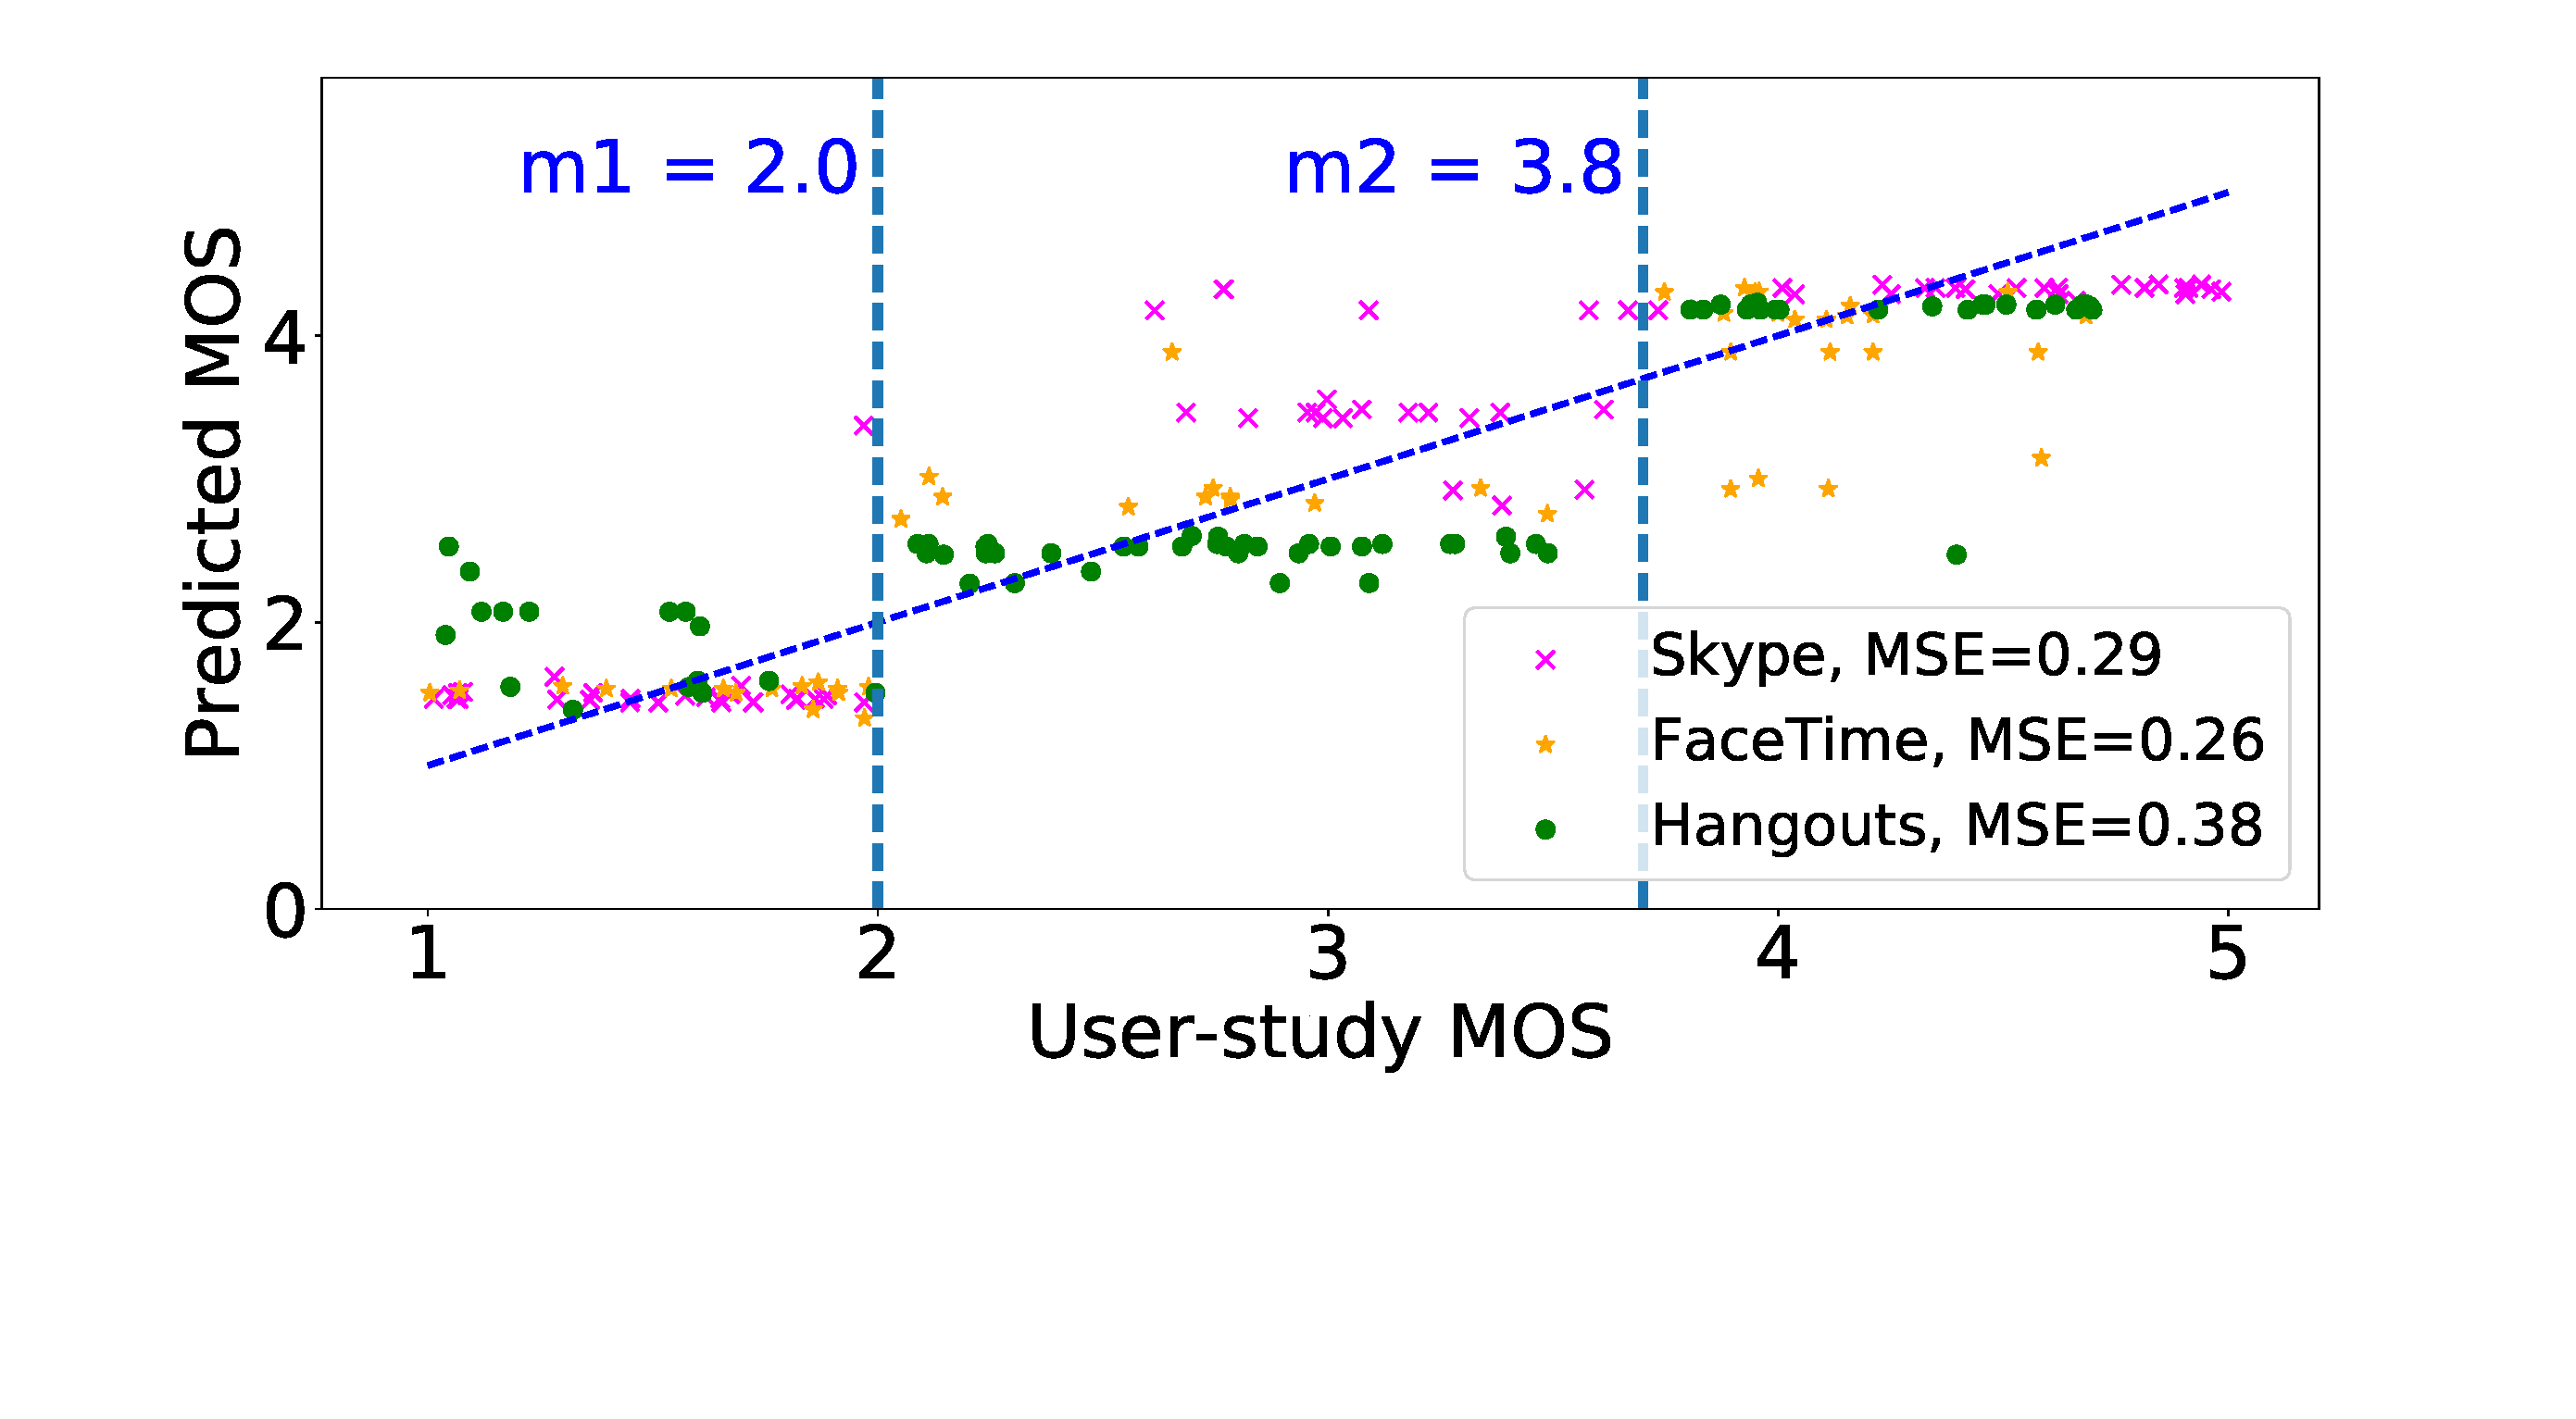
\includegraphics[width=\linewidth]{sections/network-work/scores.pdf}
      \vspace{-5em}
      \caption{User-study vs. predicted MOS for the three applications. We also show 3 clear QoE clusters divided by our thresholds $m_1=2$ and $m_2\approx 3.8.$}
      %\vspace{-1.7em}
      \label{fig:scores}
\end{figure}

Fig. \ref{fig:scores} shows a scatter plot of user-study MOS vs.~predicted MOS for the three applications. The MSE in MOS for the three applications is smaller than $0.4$ with ADT for all the applications. We also observe three clear clusters approximately divided by the MOS scores $m_1=2$ and $m_2=4$, that coincide with our thresholds for labeling the scores into 3 classes. This also justifies our design choice to finally employ three labels (bad, average, good) out of 5 MOS scores.

\noindent\textbf{Model performance for Skype:} 
Table \ref{class-skype} shows performance of Skype model across different regressors. 
The MSE in MOS is $0.29$ in case of ADT and it is $0.63$ with KNN regressor. 
Similarly, precision, accuracy and recall for ADT is the highest, while KNN being lowest.
ADT model gives a best threshold of $m_1=2$ and $m_2=3.8$ in separating the MOS scores into labels. While all the other models produce a threshold of $m_1=2$ and $m_2=3.4$.
Here, the best performance in ADT results from $(i)$ its low MSE and $(ii)$ the wide range for average class separation, i.e., it labels all the samples from MOS $2$ to $3.8$ as average class, while other models yield average class from MOS $2$ to $3.4$.
The performance gap is due to the distribution of our average class samples spread over wider range of bad or good labels. 
Using $m_1=2$ and $m_2=3.8$ thresholds, we get 30\%, 40\% and 30\% of our 300 samples in bad, average and good labels.

To show that our Skype model is device independent, we further evaluate our model across three devices: SG-S6 phone, SG-S2 Tab and Pixel Tab. Table \ref{label:skype-devices} shows precision, accuracy and recall for all three devices. We measure performance by training on one device, and testing on other devices. We observe that the performance is always better when trained and tested on the same device compared to training on one device and testing on other device. However, we find a difference of less than $7\%$ in accuracy when trained and tested across different devices, with an accuracy of at least 83\%. This corroborates that our model is robust across devices and it can be trained and tested without device constraints i.e., our metrics can collected on a certain device and can be applied to any other devices for Skype.

\noindent\textbf{Model performance for FaceTime:} 
Table \ref{class-facetime} shows performance of FaceTime model across different regressors.
Similar to Skype, we observe similar performance ($>89\%$ accuracy) for all models except the KNN regressor. 
Here, although the RF regressor is performing better ($90.37\%$ precision) than ADT, the MSE in MOS is larger than ADT.
Interestingly, all models produce same thresholds of $m_1=2$ and $m_2=3.4$ in labeling the scores.
Here, the samples are distributed uniformly across three classes unlike Skype, hence all regressors are performing almost equally. However, KNN regressor still suffers in FaceTime model due to weakness with many features as explained above. 
Using these thresholds, we get 30\%, 36\% and 34\% of the 200 samples in bad, average and good labels.

To validate that our FaceTime model is device independent, we train and test across iPad and iPhone devices.
Table \ref{label:facetime-devices} shows that when training and testing on same device, we observe $92\%$ accuracy. Whereas, training  and testing across devices yields at least $88\%$ accuracy. Hence, we observe a difference of $4\%$ accuracy across device training and testing. Our FaceTime model is also device-independent. Note that, we are not comparing the performance of our model training on Android devices and testing on iOS devices and vice-versa, because the recording set-up is different these environments.

\noindent\textbf{Model performance for Hangouts:} 
Table \ref{class-hangouts} shows performance of Hangouts model across different regressors.
Similar to other applications, ADT outperforms other models with 93.33\% accuracy with an average MSE of 0.38.
Similar to FaceTime, we observe that all models produce same thresholds of $m_1=2$ and $m_2=3.5$ in labeling the scores.
Using the above thresholds, we get 32\%, 34\% and 34\% of the 300 samples in bad, average and good labels respectively.

We further evaluate the Hangouts model across three devices: SG-S6 phone, SG-S2 Tab and Pixel Tab.
Table \ref{label:hangouts-devices} shows that an accuracy of at least 86.67\% when training and testing on same device, while inter-device train and test gives an accuracy of at least 82\%.
Overall, we observe less than 8\% accuracy difference when trained and tested across different devices. This shows that the model is independent of where training and tested are conducted.
